\documentclass[../2.tex]{subfiles}
\begin{document}

    On a graph that admits non trivial gradient and divergence,
    we can define a non trivial laplacian operator on cochains as the gradient of the divergence.
    Since we are going to represent it on chains we have that
    \[ d_1d_1^\dagger \cc{i} = \cc{i}\del_1^\dagger\del_1, \]
    which is the adjoint of $\del_1\del_1^\dagger\ch{i}$.
    Again we are fixing a canonical basis as above.

    \begin{defn}
        Let $\mc{G}$ be a graph, we define the \ii{$0$-laplacian} $\Delta_0 : C_0 \to C_0$ by 
        \[ \Delta_0 := \del_1 \del^\dagger_1.\]
    \end{defn}

    One interesting propertiy of the $0$-laplacian, see Appendix \ref{app:C}, is that the dimension of its kernel equals the connected components of the graph.\\
    To illustrate some of the properties of graphs we will refer to the graph in Fig. \ref{fig:2:3}.

    \begin{figure}[H]
        \begin{minipage}{.5\textwidth}
            \centering
            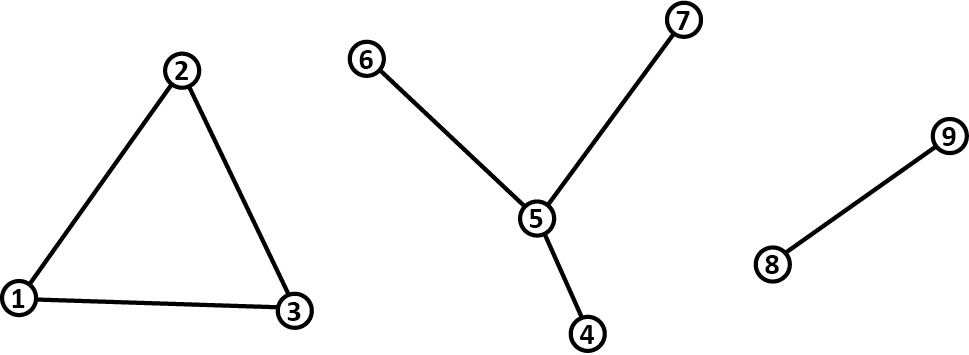
\includegraphics[width=9cm]{sections/2/graphex}
            \caption{The graph.}
            \label{fig:2:3}
        \end{minipage}
        \begin{minipage}{.5\textwidth}
            \centering
            \[\begin{pmatrix}
                0 & 1 & 1 & 0 & 0 & 0 & 0 & 0 & 0 \\
                1 & 0 & 1 & 0 & 0 & 0 & 0 & 0 & 0 \\
                1 & 1 & 0 & 0 & 0 & 0 & 0 & 0 & 0 \\
                0 & 0 & 0 & 0 & 1 & 0 & 0 & 0 & 0 \\
                0 & 0 & 0 & 1 & 0 & 1 & 1 & 0 & 0 \\
                0 & 0 & 0 & 0 & 1 & 0 & 0 & 0 & 0 \\
                0 & 0 & 0 & 0 & 1 & 0 & 0 & 0 & 0 \\
                0 & 0 & 0 & 0 & 0 & 0 & 0 & 0 & 1 \\
                0 & 0 & 0 & 0 & 0 & 0 & 0 & 1 & 0
            \end{pmatrix}. \]
            \caption{Adjacency matrix of the graph.}
            \label{fig:2:4}
        \end{minipage}
    \end{figure}

    \begin{exa}
        Let $\mc{G}$ be the graph  in \autoref{fig:2:3}, then the $0$-laplacian expressed in terms of the canoncal vertex basis $\{\ket{i}\}_{i \in I}$ is

        \[\begin{pmatrix}
                2 & -1 & -1 & 0 & 0 & 0 & 0 & 0 & 0 \\
                -1 & 2 & -1 & 0 & 0 & 0 & 0 & 0 & 0 \\
                -1 & -1 & 2 & 0 & 0 & 0 & 0 & 0 & 0 \\
                0 & 0 & 0 & 1 & -1 & 0 & 0 & 0 & 0 \\
                0 & 0 & 0 & -1 & 3 & -1 & -1 & 0 & 0 \\
                0 & 0 & 0 & 0 & -1 & 1 & 0 & 0 & 0 \\
                0 & 0 & 0 & 0 & -1 & 0 & 1 & 0 & 0 \\
                0 & 0 & 0 & 0 & 0 & 0 & 0 & 1 & -1 \\
                0 & 0 & 0 & 0 & 0 & 0 & 0 & -1 & 1 
            \end{pmatrix}. \] 

        The laplacian matrix is calculated as follows
        \[ \Delta_0 \ket{1} = \del_1\ket{1,2} + \del_1\ket{1,3} = 2\cdot\ket{1}-\ket{2}-\ket{3},\]
        \[ \Delta_0 \ket{2} = \del_1\ket{2,1} + \del_1\ket{2,3} = -\ket{1}+2\cdot\ket{2}-\ket{3},\]
        \[ \Delta_0 \ket{3} = \del_1\ket{3,1} + \del_1\ket{3,2} = -\ket{1}-\ket{2}+2\cdot\ket{3},\]
        \[ \Delta_0 \ket{4} = \del_1\ket{4,5} = \ket{4}-\ket{5},\]
        \[ \Delta_0 \ket{5} = \del_1\ket{5,4}+\del_1\ket{5,6}+\del_1\ket{5,7} = -\ket{4}+3\cdot\ket{5}-\ket{6}-\ket{7},\]
        \[ \Delta_0 \ket{6} = \del_1\ket{6,5} = -\ket{5}+\ket{6},\]
        \[ \Delta_0 \ket{7} = \del_1\ket{7,5} = -\ket{5}+\ket{7},\]
        \[ \Delta_0 \ket{8} = \del_1\ket{8,9} = \ket{8}-\ket{9},\]
        \[ \Delta_0 \ket{9} = \del_1\ket{9,8} = -\ket{8}+\ket{9}.\] 

        Three invariant subspaces emerge from the laplacian, that determine three different laplacians, namely
        \[ \Delta_0 = \Delta_0^\mc{A} \oplus \Delta_0^\mc{B} \oplus \Delta_0^\mc{C}. \]

        Furthermore any of those three blocks has a $1$-dimensional kernel, in fact the dimensional equiations for the laplacians are

        \[dim(ker\Delta_0^\mc{A}) =dimC_0(\mc{A}) - rank
        \begin{pmatrix}
            2 & -1 & -1  \\
            -1 & 2 & -1  \\
            -1 & -1 & 2 
        \end{pmatrix} = 3 - rank
        \begin{pmatrix}
            2 & 0 & -1  \\
            0 & 1 & -1  \\
            0 & 0 & 0 
        \end{pmatrix} = 3 - 2 =  1, \]

        \[ dim(ker\Delta_0^\mc{B}) =dimC_0(\mc{B}) - rank
        \begin{pmatrix}
            1 & -1 & 0 & 0  \\
            -1 & 3 & -1 & -1 \\
            0 & -1 & 1 & 0  \\
            0 & -1 & 0 & 1 
        \end{pmatrix} = 4 - rank
        \begin{pmatrix}
            1 & -1 & 0 & 0  \\
            0 & 2 & 0 & -1 \\
            0 & 0 & 1 & -1  \\
            0 & 0 & 0 & 0 
        \end{pmatrix} = 4 - 3 = 1,\]
        
        \[ dim(ker\Delta_0^\mc{C}) =dimC_0(\mc{C}) - rank
        \begin{pmatrix}
            1 & -1 \\
            -1 & 1
        \end{pmatrix} = 2 - rank
        \begin{pmatrix}
            1 & -1 \\
            0 & 0
        \end{pmatrix} = 2-1 = 1.\]
    \end{exa}

    We can also define an higher dimensional laplacian on the graph.

    \begin{defn}
        Let $\mc{G}$ be a graph, we define the \ii{$1$-laplacian} $\Delta_1 : C_1 \to C_1$ by 
        \[ \Delta_1 := \del_1^\dagger \del_1.\]
    \end{defn}

    One intersting property of the $1$-laplacian, see Appendix \ref{app:C}, is that the dimension of its kernel equals the number of independent cycles.

    \begin{exa}
        In fact we can expand $\Delta_1^\mc{A} := \del_1^\dagger\del_1$ the basis $\{\ket{1,2},\ket{2,3},\ket{3,1}\}$ as
        \[\begin{pmatrix}
            2 & -1 & -1  \\
            -1 & 2 & -1  \\
            -1& -1 & 2 
        \end{pmatrix}.\] 
        The laplacian matrix is calculated as follows
        \[\Delta_1^\mc{A}\ket{1,2} = \del_1^\dagger(\ket{1}-\ket{2}) = 2\cdot\ket{1,2}-\ket{3,1}-\ket{2,3},\]
        \[\Delta_1^\mc{A}\ket{2,3} = \del_1^\dagger(\ket{2}-\ket{3}) = -\ket{1,2}+2\cdot\ket{2,3}-\ket{3,1},\]
        \[\Delta_1^\mc{A}\ket{3,1} = \del_1^\dagger(\ket{3}-\ket{1}) = -\ket{1,2}+2\cdot\ket{3,1}-\ket{2,3}.\]

        We can notice that $\Delta_2$ has a $1$-dimensional kernel.

        \[ dim(ker\Delta_1^\mc{A}) = dimC_1(\mc{A}) - rank
            \begin{pmatrix}
                2 & -1 & 1  \\
                -1 & 2 & 1  \\
                1& 1 & 2 
            \end{pmatrix} = 3 - rank
            \begin{pmatrix}
                2 & 0 & -1  \\
                0 & 1 & -1  \\
                0 & 0 & 0 
            \end{pmatrix} = 3 - 2 =  1. \]

        Since the sum of the three raws is $0$ we can say that the only linearly independent $1$-cycle is $\ket{1,2}+\ket{2,3}+\ket{3,1}$.
    \end{exa}
\end{document}